\documentclass[aps,pra,twocolumn]{revtex4-2}
\usepackage{amsmath,amsfonts,amsthm,bbm}
\usepackage[dvipsnames]{xcolor}
\usepackage{graphicx}
\usepackage{multirow,mhchem,chemformula}
\usepackage[colorlinks=true,breaklinks=true,linkcolor=red,citecolor=magenta,urlcolor=magenta]{hyperref}

\usepackage{tikz}
\usetikzlibrary{quantikz}

\newcommand{\OHradical}{\ch{OH}^\bullet}
\newcommand{\OHanion}{\ch{OH}^-}
\newcommand{\crt}[1]{\hat{c}_{#1}^\dagger}
\newcommand{\dst}[1]{\hat{c}_{#1}^{\phantom{\dagger}}}
\newcommand*\vett[1]{{\bf{#1}}}

\begin{document}

\title{$N$-electron valence perturbation theory with reference wavefunctions from quantum computing:
application to the relative stability of hydroxide ion and hydroxyl radical}

\author{Alessandro Tammaro}
\affiliation{Universit\`a degli Studi di Milano, Dipartimento di Fisica ``Aldo Pontremoli'', via Celoria 16, I-20133 Milano, Italy}
\author{Davide E. Galli}
\affiliation{Universit\`a degli Studi di Milano, Dipartimento di Fisica ``Aldo Pontremoli'', via Celoria 16, I-20133 Milano, Italy}
\author{Mario Motta}
\affiliation{IBM Quantum, IBM Research Almaden, 650 Harry Road, San Jose, CA 95120, USA}

\begin{abstract}
Quantum simulations of the hydroxide ion and hydroxyl radical are reported, employing variational quantum algorithms for near-term quantum devices.
The energy of each species is calculated along the dissociation curve, to obtain information about the stability of the molecular species being investigated. 
It is shown that simulations restricted to valence spaces incorrectly predict the hydroxyl radical to be more stable than the hydroxide ion.
Inclusion of dynamical electron correlation from non-valence orbitals is demonstrated,
through the integration of the variational quantum eigensolver and quantum subspace expansion methods in the workflow of $N$-electron valence perturbation theory, 
and shown to correctly predict the hydroxide ion to be more stable than the hydroxyl radical, provided that basis sets with diffuse orbitals are employed.
\end{abstract}

\maketitle

\section{Introduction}

The simulation of many-body quantum systems is an important application for a quantum computer \cite{georgescu2014quantum,cao2019quantum,cerezo2020variational,bauer2020quantum,mcardle2020quantum,motta2021emerging}. 
In the context of quantum chemistry, an important example of such an application is the electronic structure problem, 
namely solving for the ground or low-lying eigenstates of the electronic Schr\"{o}dinger equation for the Born-Oppenheimer hamiltonian \cite{friesner2005ab,helgaker2012recent,helgaker2014molecular}.

In recent years, a variety of quantum algorithms has delivered promising results in the calculation of potential energy curves,
ground- and excited-state energies and ground-state correlation functions for a variety of molecules \cite{cao2019quantum,cerezo2020variational,bauer2020quantum,mcardle2020quantum,motta2021emerging}.
Notwithstanding this progress, the limitations of contemporary quantum computation platforms 
have resulted in most quantum electronic structure simulations reported to date employing minimal basis sets (i.e. describing core and valence orbitals only)
or being restricted to active spaces of a few orbitals and electrons.
While these simulations include some electronic correlation, thanks to the ability to entangle electrons within the active space, 
the dynamical correlation arising from inactive orbitals is important to obtain quantitatively and qualitatively correct results.

In recent years, a number of hybrid quantum-classical algorithms have been proposed, 
which aim to combine simulations on contemporary quantum computation platforms with pre- and post-processing operations carried out on classical computers, 
in order to achieve more expressive computations
\cite{bravyi2016trading,kreula2016few,yamazaki2018towards,peng2020simulating,takeshita2020increasing,kawashima2021optimizing,mitarai2021constructing,yuan2021quantum,eddins2021doubling}.

In the present work, we integrate the variational quantum eigensolver (VQE) \cite{farhi2014quantum,peruzzo2014variational,mcclean2016theory,romero2018strategies}
and quantum subspace expansion (QSE) \cite{mcclean2017hybrid,colless2018computation,huggins2020non}
methods in the workflow of N-electron valence perturbation theory (NEVPT2) \cite{angeli2001introduction,angeli2001n,sokolov2016time,sokolov2017time}.

The combination of VQE and QSE allows to produce approximations for the ground and excited states of the Born-Oppenheimer hamiltonian within an active space
based on intrinsic atomic orbitals (IAOs) \cite{knizia2013intrinsic,senjean2020generalization,schwilkIAO,ManzIAO,WestIAO,ElviraIAO,SchneiderIAO,barison2020quantum}, a
nd comprising valence orbitals and electrons.
Information from these calculations is then used to compute a perturbative correction to the ground-state energy provided by VQE,
that accounts for one- and two-electron transitions from active to inactive orbitals.
We apply the NEVPT2 formalism to examine the relative stability of the hydroxide ion and hydroxyl radical. 
We observe that valence-only simulations incorrectly predict the radical to have lower energy than the anion. 
Further, we observe that inclusion of dynamical electron correlation from non-valence orbitals leads to correctly predicting that the hydroxide ion is more stable
than the hydroxyl radical, when basis sets with diffuse orbitals are employed.

The remainder of the present work is organized as follows. The NEVPT2 formalism and its integration with VQE and QSE are described in Section \ref{sec:methods}.
Results are presented in Section \ref{sec:results}, and conclusions are drawn in Section \ref{sec:conclusions}. An appendix reports additional computational details,
and the source code used to generate the data presented in this study can be publicly accessed on GitHub at \cite{tammaro2022github}.

\section{Methods}
\label{sec:methods}

We begin with a brief overview of multi-reference perturbation theory, and an instructional account of the working equations used in the present study. 
Our starting point is the Born-Oppenheimer Hamiltonian written in second quantization,
\begin{equation}
\hat{H} = E_0 + \sum_{\substack{pr \\ \sigma}} h_{pr} \crt{p\sigma} \dst{r\sigma} + \sum_{\substack{prqs \\ \sigma\tau}} \frac{(pr|qs)}{2} \crt{p\sigma} \crt{q\tau} \dst{s\tau}  \dst{r\sigma} 
\quad,
\end{equation}
where indices $p,r,q,s$ label spatial orbitals in a finite orthonormal basis, and $\sigma,\tau \in \{ \uparrow,\downarrow \}$ are spin indices. The constant 
\begin{equation}
E_0 = \sum_{a<b=1}^{N_n} \frac{Z_a Z_b}{| \vett{R}_a - \vett{R}_b|} \quad,
\end{equation}
where $\vett{R}_a$ and $Z_a$ are the position and atomic number of nucleus $a$, describes the nucleus-nucleus Coulomb interaction.
The coefficients 
\begin{equation}
h_{pr} = \int d {\bf{x}} \, \varphi_p({\bf{x}}) \, \left[ - \frac{1}{2} \, \frac{\partial^2}{\partial \vett{r}}  - \sum_{a=1}^{N_n} \frac{Z_a}{| \vett{r} - \vett{R}_a |} \right] \, \varphi_r({\bf{x}})
\quad,
\end{equation}
describes the one-electron part of the Hamiltonian, and
\begin{equation}
(pr|qs) = \int d {\bf{x}} \int d {\bf{y}} \,  \frac{ \varphi_p({\bf{x}}) \varphi_r({\bf{x}}) \, \varphi_q({\bf{y}}) \varphi_s({\bf{y}}) }{ |\vett{x} - \vett{y} | }
\end{equation}
describes the electron-electron Coulomb interaction. 
Hartree units are used thorough, the numbers of spin-up and spin-down electrons and nuclei are $N_\uparrow$, $N_\downarrow$, and $N_n$ respectively,
and orbitals $\varphi_p$ are assumed real-valued, which ensures $(pr|qs)$ has 8-fold symmetry.

Following published literature \cite{sokolov2016time,sokolov2017time}, we partition the spatial orbitals into three sets:
(i) core (doubly-occupied) with indices $i,j,k,l$ 
(ii) active with indices $u,v,w,x,y,z$ and 
(iii) external (unoccupied) with indices $a,b,c,d$. 
We construct core, active, and external orbitals with a procedure based on the formalism of IAOs \cite{knizia2013intrinsic}, detailed in Appendix \ref{app:orbitals}.
Core orbitals are frozen, leading to the transformed Hamiltonian
\begin{equation}
\label{eq:core_frozen}
\hat{H} = E_0^\prime + \sum_{\substack{pr \\ \sigma}} t_{pr} \crt{p\sigma} \dst{r\sigma} + \sum_{\substack{prqs \\ \sigma\tau}} \frac{v_{prqs}}{2} \crt{p\sigma} \crt{q\tau} \dst{s\tau}  \dst{r\sigma}
\end{equation}
where the coefficients $E_0^\prime$, $t_{pr}$ and $v_{prqs}$ are detailed in Appendix \ref{app:core} and the indices $p,r,q,s$ will be henceforth used to indicate
active and external orbitals. The Hamiltonian is written as the sum of a Dyall operator \cite{dyall1995choice},
\begin{equation}
\label{eq:dyall}
\hat{H}_d = \sum_{\substack{a \\ \sigma}} \varepsilon_a \, \crt{a\sigma} \dst{a\sigma} + \hat{H}_{act} \quad,
\end{equation}
and of a perturbation $\hat{V} = \hat{H} - \hat{H}_d$. 
In Eq.~\eqref{eq:dyall}, the orbital energies $\varepsilon_a$ are defined as the eigenvalues of the projection of the Fock operator $\hat{F}$ on the external space, and
\begin{equation}
\hat{H}_{act} = E_0^\prime + \sum_{\substack{uv \\ \sigma}} t_{uv} \crt{u\sigma} \dst{v\sigma} 
+ \sum_{\substack{uvwx \\\sigma\tau}} \frac{v_{uvwx}}{2} \crt{u\sigma} \crt{w\tau} \dst{x\tau}  \dst{v\sigma}
\end{equation}
is the restriction of the Born-Oppenheimer Hamiltonian to the active space.
The second-order energy contribution can be written as
\begin{equation}
\label{eq:nevpt2}
- E_2 = \sum_{\mu \neq 0} \frac{| \langle \Psi_\mu | \hat{V} | \Psi_0 \rangle |^2}{E_\mu - E_0}
\end{equation}
where $(\Psi_\mu,E_\mu)$ are the eigenpairs of the Dyall Hamiltonian $\hat{H}_d$, and in particular $\mu=0$ corresponds to the ground state. 
Eq~\eqref{eq:nevpt2} is the second-order energy expression from the Rayleigh-Schr\"{o}dinger perturbation theory,
which yields the exact energy of the second-order $N$-electron valence perturbation theory (NEVPT2) \cite{angeli2001introduction,angeli2001n,sokolov2016time,sokolov2017time}.

In order to evaluate Eq.~\eqref{eq:nevpt2}, it is necessary to know all the eigenvalues and eigenvectors of the Dyall Hamiltonian 
such that $\langle \Psi_\mu | \hat{V} | \Psi_0 \rangle \neq 0$. To elucidate the structure of such eigenstates, it is useful to recall
that the action of $\hat{V}$ over the ground state reads
\begin{equation}
\label{eq:nevpt3}
\begin{split}
\hat{V} | \Psi_0 \rangle 
&= 
\Bigg[ \sum_{\substack{a \\ \sigma}} \crt{a\sigma} \hat{O}^{(1)}_{a,\sigma} + \sum_{\substack{a<b \\ \sigma}} \crt{a\sigma}\crt{b\sigma} \hat{O}^{(2)}_{ab,\sigma} \\
&+ 
\sum_{ab} \crt{a\uparrow} \crt{b\downarrow} \hat{O}^{(3)}_{ab} \Bigg] | \Psi_0 \rangle \\
\end{split}
\end{equation}
where the operators
\begin{equation}
\label{eq:nevpt4}
\begin{split}
\hat{O}^{(1)}_{a,\sigma} &= \sum_{y} t_{ay} \, \dst{y\sigma} + \sum_{ \substack{ywz \\ \tau} } v_{aywz} \, \crt{w\tau} \dst{z\tau} \dst{y\sigma} \quad, \\
\hat{O}^{(2)}_{ab,\sigma} &= \sum_{xy} v_{aybx} \, \dst{x\sigma}  \dst{y\sigma} \quad, \\
\hat{O}^{(3)}_{ab} &= \sum_{xy} v_{aybx} \, \dst{x\downarrow}  \dst{y\uparrow} \quad, \\
\end{split}
\end{equation}
respectively remove a particle with spin $\sigma$, two particles with identical spins $\sigma$, and two particles with opposite spin from the active space.
In the light of Eq.~\eqref{eq:nevpt4}, Eq.~\eqref{eq:nevpt3} takes the form
\begin{equation}
\begin{split}
\label{eq:nevpt5}
- E_2 
&= \sum_{\mu} \sum_{\substack{a \\ \sigma}} 
\;
\frac{| \langle \Phi^{(\sigma)}_\mu | \hat{O}^{(1)}_{a,\sigma} | \Phi_0 \rangle |^2}{\varepsilon_a + \tilde{E}^\sigma_\mu - \tilde{E}_0} \\
&+ \sum_{\mu} \sum_{\substack{a<b \\ \sigma}} 
\;
\frac{| \langle \Phi^{(\sigma\sigma)}_\mu | \hat{O}^{(2)}_{ab,\sigma} | \Phi_0 \rangle |^2}{\varepsilon_a + \varepsilon_{b} + \tilde{E}^{\sigma\sigma}_\mu - \tilde{E}_0} \\
&+ \sum_{\mu} \sum_{ab} 
\;
\frac{| \langle \Phi^{(\uparrow\downarrow)}_\mu | \hat{O}^{(3)}_{ab} | \Phi_0 \rangle |^2}{\varepsilon_a + \varepsilon_{b} + \tilde{E}^{\uparrow\downarrow}_\mu - \tilde{E}_0} \\
\end{split}
\end{equation}
where 
$(\Phi_\mu^{(\uparrow)},\tilde{E}^{(\uparrow)}_\mu)$
denotes the eigenpairs of the active-space Hamiltonian $\hat{H}_{act}$ 
in the sector of the Fock space with 
$(N_\uparrow-1,N_\downarrow)$ particles, etc.

Unlike Eq.~\eqref{eq:nevpt3}, the last expression for the correlation energy involves solutions of the Schr\"{o}dinger equation in the active space.
A natural way to approximately evaluate Eq.~\eqref{eq:nevpt5} is to integrate the variational quantum eigensolver (VQE) 
and quantum subspace expansion methods (QSE) in the workflow of NEVPT2. More specifically, 

(i) an initial VQE calculation is performed, to approximate the ground state of $\hat{H}_{act}$; (ii) then, we formulate the following Ans\"{a}tze for the excited states,
\begin{equation}
\label{eq:nevpt6}
\begin{split}
| \Phi^\sigma_{\mu} \rangle &= \sum_u \chi^\sigma_{u,\mu} \dst{u\sigma} | \Phi_0 \rangle \quad, \\
| \Phi^{\sigma\sigma}_{\mu} \rangle &= \sum_{u<v} \chi^{\sigma\sigma}_{uv,\mu} \dst{u\sigma} \dst{v\sigma} | \Phi_0 \rangle \quad, \\
| \Phi^{\uparrow\downarrow}_{\mu} \rangle &= \sum_{uv} \chi^{\uparrow\downarrow}_{uv,\mu} \dst{u\uparrow} \dst{v\downarrow} | \Phi_0 \rangle \quad. \\
\end{split}
\end{equation}
In the forthcoming equations, the states \eqref{eq:nevpt6} will be compactly denoted as $| \Phi_\mu \rangle = \sum_\alpha \chi_{\alpha,\mu} \, \hat{E}_\alpha | \Phi_0 \rangle$;

(iii) the coefficients $\chi_{\alpha,\mu}$ are evaluated by forming the overlap and Hamiltonian matrices
\begin{equation}
\label{eq:nevpt7}
\begin{split}
S_{\alpha\beta} &= \langle \Phi_0 | \hat{E}_\alpha^\dagger \hat{E}_\beta | \Phi_0 \rangle \quad, \\
H_{\alpha\beta} &= \langle \Phi_0 | \hat{E}_\alpha^\dagger \hat{H}_{act} \hat{E}_\beta | \Phi_0 \rangle \quad, \\
\end{split}
\end{equation}
and diagonalizing them, $\sum_\beta H_{\alpha\beta} \chi_{\beta,\mu} = \tilde{E}_\mu \sum_\beta S_{\alpha\beta} \chi_{\beta,\mu}$;

(iv) the transition matrix elements appearing in Eq.~\eqref{eq:nevpt5} are computed from the coefficients $\chi_{\alpha,\mu}$ and the overlap matrices $S_{\alpha\beta}$
with the formulas reported in Appendix \ref{app:transition}, and Eq.~\eqref{eq:nevpt5} is evaluated.

\subsection{Computational cost and accuracy limitations}

The computational cost of the procedure outlined in the previous Section is 
$\mathcal{O}(N_{act}^4 N_{qse}^2)$ Pauli measurements to synthesize the matrices in Eq.~\eqref{eq:nevpt7},
$\mathcal{O}(N_{qse}^3)$ to diagonalize them and obtain the coefficients $\chi_{\alpha,\mu}$, 
$\mathcal{O}(N^2_{ext} N^2_{act} N_{qse})$ to compute the transition matrix elements appearing in Eq.~\eqref{eq:nevpt5} as explained in Appendix \ref{app:transition}, 
and $\mathcal{O}(N_{qse} N_{ext}^2)$ to compute the correlation energy. 
The Ansatz Eq.~\eqref{eq:nevpt6} is designed to maintain the computational cost of QSE as low as possible, and in particular $N_{qse} = \mathcal{O}(N_{act}^2)$.
However, it introduces two approximations with respect to NEVPT2: 
first, the replacement of the exact ground state (GS) with a VQE Ansatz; second, the retention of a limited number of excited states (ES).
In the remainder of this work, we endeavor to assess the impact of both approximations on the final results, by comparing:

(i) NEVPT2 with exact GS and exact ES, denoted NEVPT2(FCI,FCI), 

(ii) NEVPT2 with exact GS and ES approximated by Eq.~\eqref{eq:nevpt6}, denoted NEVPT2(FCI,QSE), 

(iii) NEVPT2 with VQE Ansatz and ES approximated by Eq.~\eqref{eq:nevpt6}, denoted NEVPT2(Ansatz,QSE).

Comparison (i) versus (ii) and (ii) versus (iii) permits to assess the impact of the QSE and VQE approximations on the accuracy of NEVPT2 respectively.

\subsection{Additional computational details}

The calculations performed in this work involved initial pre-processing by the quantum chemistry codePySCF \cite{sun2018pyscf,sun2020recent}) 
on classical computers, to generate optimized mean-field orbitals and Hamiltonian coefficients prior to performing computations with quantum simulators. 
The restricted closed- and open-shell Hartree-Fock (RHF, ROHF) states were chosen as the initial states for all of the calculations described here. 
All correlated calculations used the frozen core approximation, and the lowest $N_{core}=2$ MOs were frozen, for the purpose of economizing simulations.
This lead to $N_{act} = 4$ and $N_{ext}$ ranging between 5 and 120 (respectively 6-31G and aug-cc-pVQZ).

Having selected a set of single-electron orbitals for each of the studied species, VQE computations were performed with quantum simulators.
We used IBM's open-source library for quantum computing, Qiskit \cite{aleksandrowicz2019qiskit}.
Qiskit Aqua contains implementations of techniques to map the fermionic Fock space onto the Hilbert space of a register of qubits, and an implementation of the VQE algorithm.
Here we use the tapering-off technique \cite{bravyi2017tapering,setia2019reducing} to account for molecular point group symmetries and reduce the number of qubits required for a simulation. 
In analogy with conventional symmetry-adapted quantum chemistry calculations, this reduction does not introduce additional approximations in the calculations.
For the problems considered here, the tapering-off technique reduced the number of qubits to $n_q=4$.

In the VQE algorithm, we take our wavefunction in the form of a quantum circuit, which is the quantum unitary coupled cluster with singles 
and doubles q-UCCSD \cite{barkoutsos2018quantum}, and the following $R_y$ Ansatz,
\begin{equation}
\begin{split}
| \Psi(\theta) \rangle &= 
\prod_{k=1}^{n_r}
\left[
\prod_{i=0}^{n_q-1} R^{i}_{y}(\theta_{k}^i)
E
\right]
\prod_{i=0}^{n_q-1} R^{i}_{y}(\theta_{0}^i) | \Psi_0 \rangle
\;, \\
E &= \prod_{ij\in C} G_{ij} \;,
\end{split}
\end{equation}
where $| \Psi_0 \rangle$ is an initial wavefunction (here, the restricted closed- or open-shell Hartree-Fock state), $m$ is the number of qubits, $R^i_{y}(\theta) 
= \mbox{exp}(-i \theta Y_i/2)$ is a $Y$ rotation of an angle $\theta$ applied to qubit $i$, $G_{ij}$ a parameter-free two-qubit entangling gate (here, the CNOT gate) 
applied to a pair $(ij)$ of connected qubits (here, we chose linear connectivity, i.e. $(ij) \in C$ if and only if $j=i+1$),
and $n_r$ is an integer denoting the number of times a layer of entangling gates followed by a layer of $Y$ rotations is repeated. 
In this study, to ensure an accurate representation of the ground-state wavefunction by the $R_y$ Ansatz, we chose $n_r = 3$, corresponding to the quantum circuit shown in Appendix \ref{app:ry}.

We then minimized the expectation value of the Hamiltonian with respect to the parameters in the circuit. 
The minimization was carried out using the classical optimization method, L-BFGS-B \cite{zhu1997algorithm,morales2011remark}. 
We ran our experiments on the ideal and noiseless statevector simulator of Qiskit.
Once the VQE is complete, we obtain the optimized variational form and the estimate for the ground state energy. 
In addition, we measure the operators corresponding to the QSE overlap and Hamiltonian matrices using standard functionalities.

%%%%%%%%%%%%%%%%%%%%%%%%%%%%%%%%%%%%%%%%%%%%%%%% POPLE FIG

\begin{figure*}[t!]
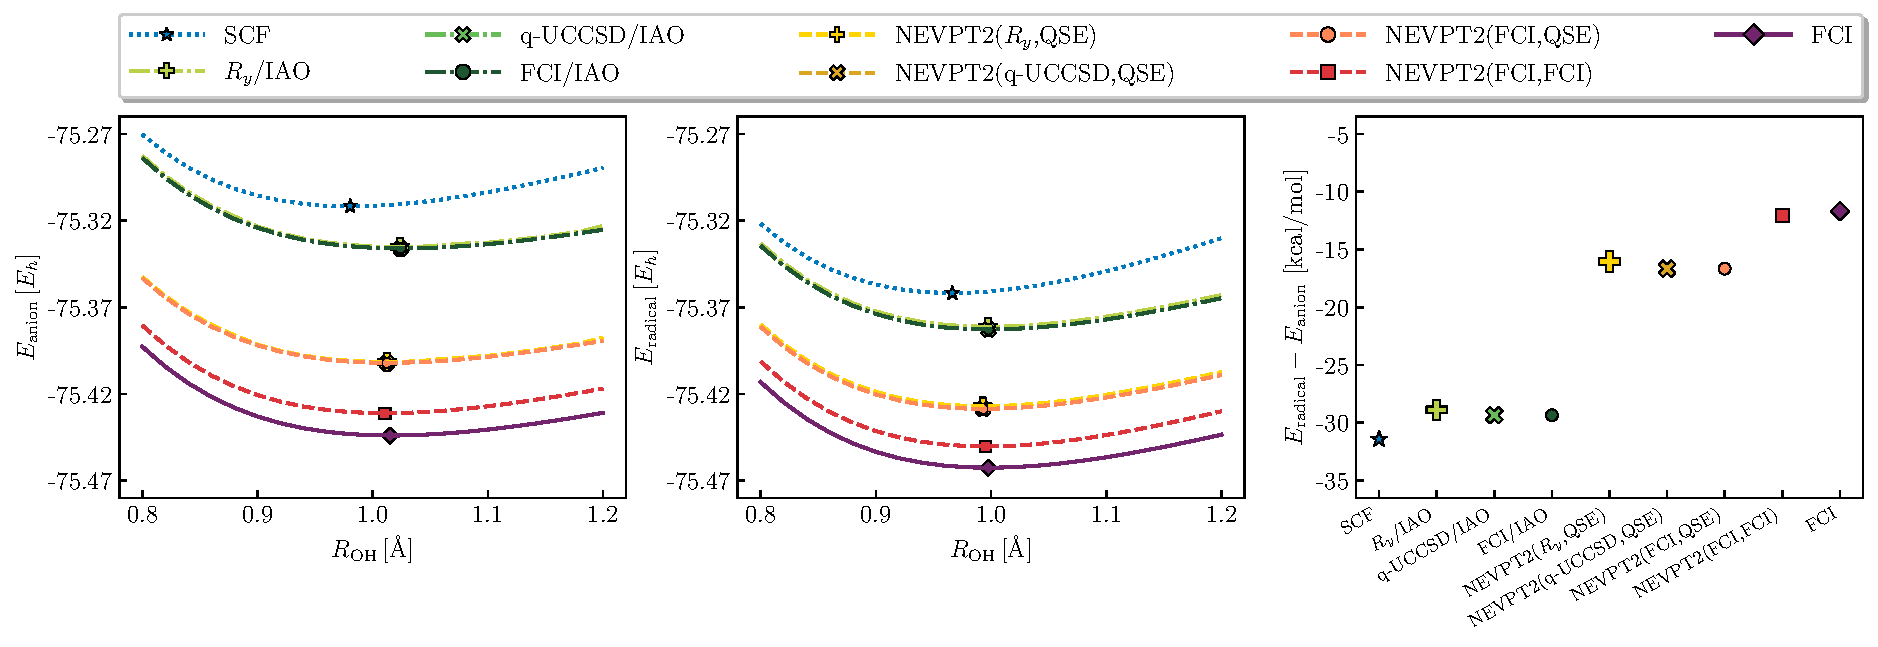
\includegraphics[width=\textwidth]{../nevpt2/6-31g/fig.pdf}
\caption{Left: potential energy curve of $\OHanion$ (anion)
from SCF (blue dotted line),
VQE and FCI in the IAO basis computed from an underlying 6-31G basis (green dash-dotted lines),
and various approximations of NEVPT2 (warm colored dashed lines), and FCI in the underlying 6-31G basis (purple solid line).
Symbols denote equilibrium geometries and energies from a fit to a Morse potential.
Middle: same as left, for $\OHradical$ (radical).
Right: Ground-state energy difference between anion and radical.}
\label{figure:631g}
\end{figure*}

\begin{figure*}[t!]
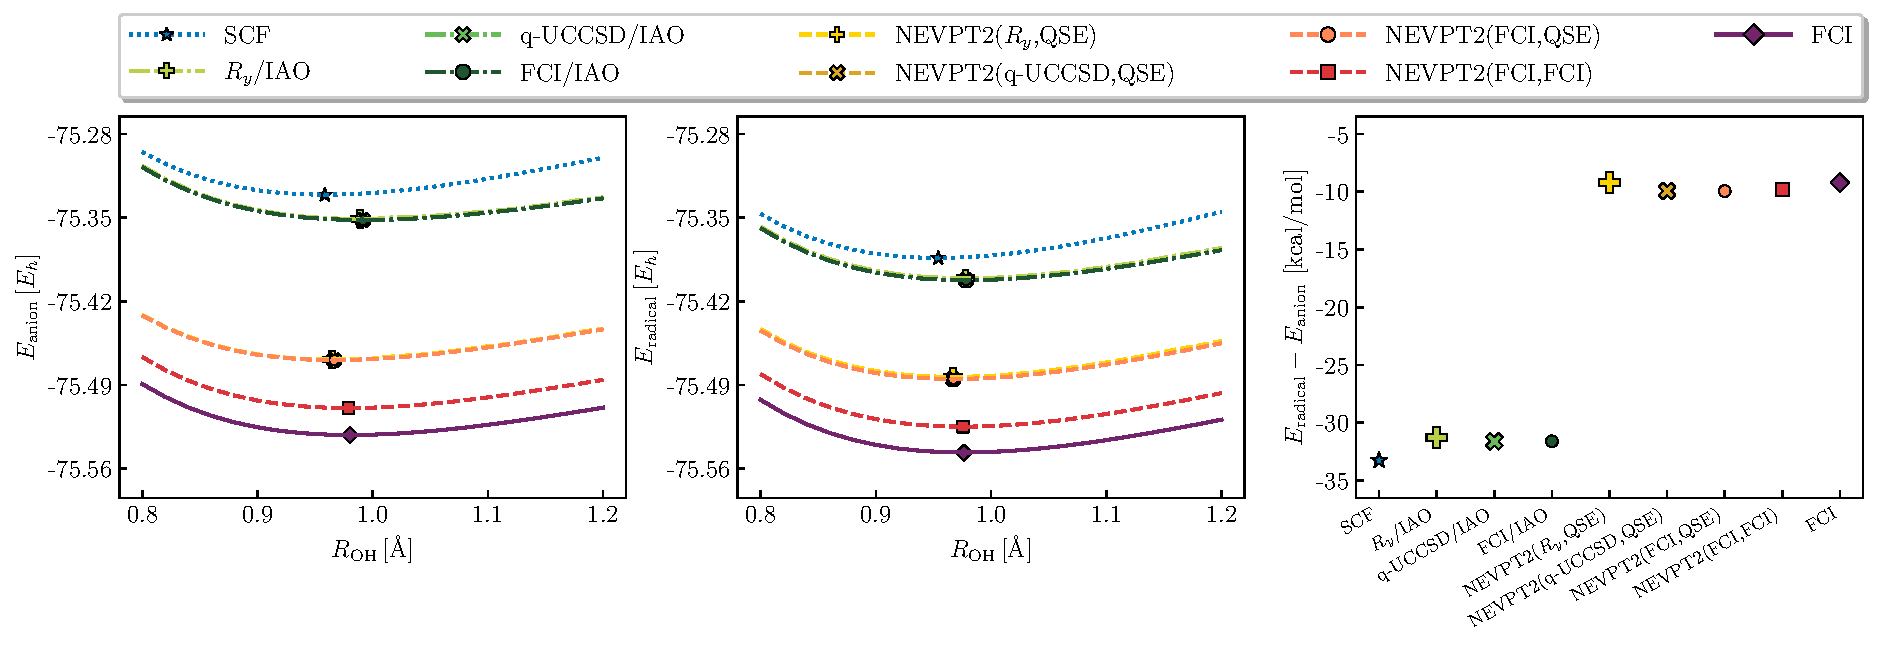
\includegraphics[width=\textwidth]{../nevpt2/6-31gss/fig.pdf}
\caption{Same as Fig~\ref{figure:631g} using an underlying 6-31G${}^{**}$ basis.}
\label{figure:631gss}
\end{figure*}

\section{Results}
\label{sec:results}

In this section, we simulate the hydroxide ion ($\OHanion$) and hydroxyl radical ($\OHradical$) using split-valence 6-31G, 6-31G${}^{**}$, 6-31G++, and 6-31$++$G${}^{**}$ basis sets
\cite{hehre1972self} and correlation-consistent aug-cc-pVxZ basis sets \cite{dunning1989gaussian}.
For each species, we compute the potential energy curve, namely the ground-state energy as a function of the $\ce{OH}$ bondlength $R_{\mathrm{OH}}$.
We focus on the interval $0.8 \, \mathrm{\AA} \leq R_{\mathrm{OH}} \leq 1.2 \, \mathrm{\AA}$ due to its proximity with the experimental gas-phase equilibrium bondlengths of $\OHanion$ and $\OHradical$,
respectively $R_{\mathrm{anion}} = 0.964 \, \mathrm{\AA}$ and $R_{\mathrm{radical}} = 0.970 \, \mathrm{\AA}$ \cite{johnson1999nist}.
For each species, we fit the computed potential energy curve to the Morse potential functional form, 
and extract the equilibrium bondlength $R_{eq} = \mathrm{argmin}_R E(R)$ and the equilibrium ground-state energy $E_{min} = E(R_{eq})$.
We use this information to compute the ground-state energy difference between radical and anion, 
\begin{equation}
\Delta E = E_{\mathrm{radical}}(R_{eq,\mathrm{radical}}) - E_{\mathrm{anion}}(R_{eq,\mathrm{anion}})
\quad.
\end{equation}
We compare the computed energy difference $\Delta E$ with the electron affinity of the hydroxyl radical, defined as $\OHradical(g) + e^- \to \OHanion(g) + \mathrm{EA}$,
and given by $\mathrm{EA} = 1.828 \, \mathrm{eV} = 42.1547 \, \mathrm{kcal/mol}$ \cite{johnson1999nist}.

%%%%%%%%%%%%%%%%%%%%%%%%%%%%%%%%%%%%%%%%%%%%%%%% POPLE FIG

\begin{figure*}[t!]
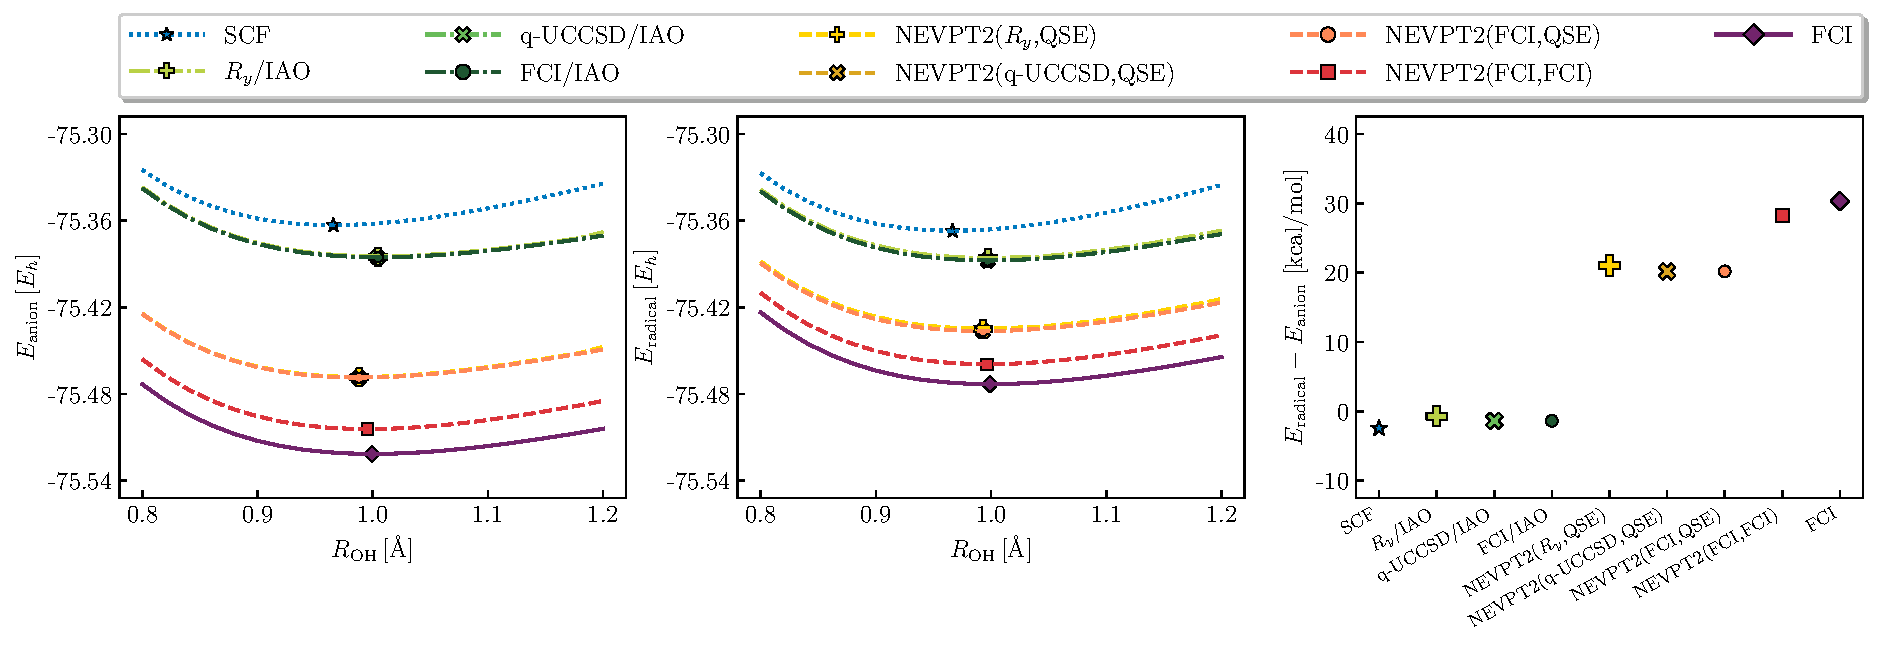
\includegraphics[width=\textwidth]{../nevpt2/6-31ppg/fig.pdf}
\caption{Same as Fig~\ref{figure:631g} using an underlying 6-31++G basis.}
\label{figure:631ppg}
\end{figure*}

\begin{figure*}[t!]
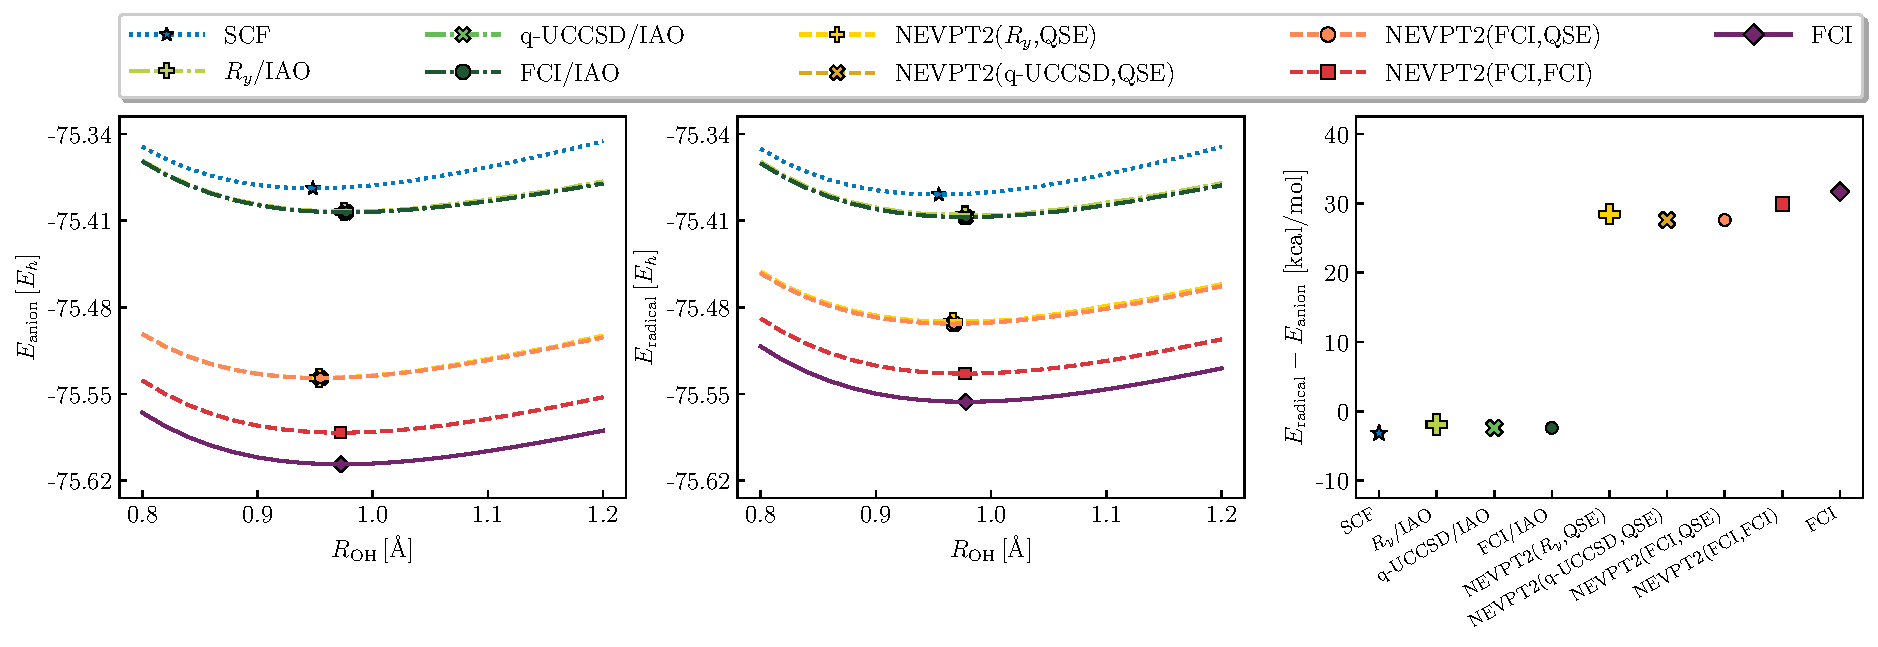
\includegraphics[width=\textwidth]{../nevpt2/6-31ppgss/fig.pdf}
\caption{Same as Fig~\ref{figure:631g} using an underlying 6-31++G${}^{**}$ basis.}
\label{figure:631ppgss}
\end{figure*}

%%%%%%%%%%%%%%%%%%%%%%%%%%%%%%%%%%%%%%%%%%%%%%%% 
 
\begin{table*}[t!]
\begin{tabular}{lccc}
\hline\hline
method & $R_{\mathrm{anion}} [\mathrm{\AA}]$ & $R_{\mathrm{radical}} [\mathrm{\AA}]$ & $\Delta E$ [kcal/mol] \\ \hline
SCF & 0.98055(16) & 0.96635(20) & -31.410(21) \\ \hline
$R_y$/IAO & 1.03610(58) & 0.99902(31) & -27.730(46) \\
q-UCCSD/IAO & 1.03646(29) & 0.99928(12) & -27.646(22) \\
FCI/IAO & 1.03646(29) & 0.99928(12) & -27.646(22) \\ \hline
NEVPT2($R_y$,QSE) & 1.01097(26) & 0.99020(14) & -16.688(21) \\
NEVPT2(q-UCCSD,QSE) & 1.01134(22) & 0.99029(11) & -16.661(17) \\
NEVPT2(FCI,QSE) & 1.01134(22) & 0.99030(11) & -16.668(17) \\
NEVPT2(FCI,FCI) & 1.02580(18) & 1.00078(15) & -13.621(18) \\ \hline
FCI & 1.02187(21) & 0.99753(15) & -13.027(19) \\
\hline\hline
\end{tabular}
\caption{Equilibrium bondlengths for $\OHanion$ (anion) and  $\OHradical$ (radical), and energy difference between anion and radical, using the methods in Fig~\ref{figure:631g} and an underlying 6-31G basis.
Values of $R_{\mathrm{anion}}$ and $R_{\mathrm{radical}}$ reflect the location of symbols in Fig~\ref{figure:631g}, left and middle panels. 
Values of $\Delta E$ corresponds to the values shown in the right panel of Fig~\ref{figure:631g}.}
\label{tab:631g}
\end{table*}


\begin{table*}[t!]
\begin{tabular}{lccc}
\hline\hline
method & $R_{\mathrm{anion}} [\mathrm{\AA}]$ & $R_{\mathrm{radical}} [\mathrm{\AA}]$ & $\Delta E$ [kcal/mol] \\ \hline
SCF & 0.95840(11) & 0.95415(18) & -33.249(20) \\ \hline
$R_y$/IAO & 0.99833(44) & 0.97758(38) & -30.320(41) \\
q-UCCSD/IAO & 0.99761(21) & 0.97775(11) & -30.321(16) \\
FCI/IAO & 0.99761(21) & 0.97775(11) & -30.321(16) \\ \hline
NEVPT2($R_y$,QSE) & 0.96922(15) & 0.96694(18) & -9.840(18) \\
NEVPT2(q-UCCSD,QSE) & 0.96905(14) & 0.96702(11) & -9.864(13) \\
NEVPT2(FCI,QSE) & 0.96905(14) & 0.96703(11) & -9.873(13) \\
NEVPT2(FCI,FCI) & 0.98082(10) & 0.97424(15) & -6.439(14) \\ \hline
FCI & 0.97754(14) & 0.97113(13) & -5.232(15) \\
\hline\hline
\end{tabular}
\caption{Same as Table~\ref{tab:631g} using an underlying 6-31G${}^{**}$ basis.}
\label{tab:631gss}
\end{table*}


\begin{table*}[t!]
\begin{tabular}{lccc}
\hline\hline
method & $R_{\mathrm{anion}} [\mathrm{\AA}]$ & $R_{\mathrm{radical}} [\mathrm{\AA}]$ & $\Delta E$ [kcal/mol] \\ \hline
SCF & 0.96596(16) & 0.96661(22) & -2.450(23) \\ \hline
$R_y$/IAO & 1.01132(59) & 0.99776(30) & -0.425(46) \\
q-UCCSD/IAO & 1.01100(23) & 0.99822(15) & -0.295(19) \\
FCI/IAO & 1.01100(23) & 0.99822(15) & -0.295(19) \\ \hline
NEVPT2($R_y$,QSE) & 0.98357(17) & 0.98977(15) & 19.074(16) \\
NEVPT2(q-UCCSD,QSE) & 0.98386(16) & 0.98966(14) & 19.068(15) \\
NEVPT2(FCI,QSE) & 0.98386(16) & 0.98966(14) & 19.060(15) \\
NEVPT2(FCI,FCI) & 1.00725(19) & 1.00183(18) & 23.998(20) \\ \hline
FCI & 1.00066(19) & 0.99838(18) & 26.979(19) \\
\hline\hline
\end{tabular}
\caption{Same as Table~\ref{tab:631g} using an underlying 6-31++G basis. 
The change in the sign of $\Delta E$ indicates the anion is predicted to be more stable than the radical when the full basis is used in NEVPT2 or FCI simulations.}
\label{tab:631ppg}
\end{table*}

\begin{table*}[t!]
\begin{tabular}{lccc}
\hline\hline
method & $R_{\mathrm{anion}} [\mathrm{\AA}]$ & $R_{\mathrm{radical}} [\mathrm{\AA}]$ & $\Delta E$ [kcal/mol] \\ \hline
SCF & 0.94806(9) & 0.95462(19) & -3.161(20) \\ \hline
$R_y$/IAO & 0.97895(29) & 0.97658(48) & -1.445(42) \\
q-UCCSD/IAO & 0.97890(12) & 0.97726(13) & -1.518(13) \\
FCI/IAO & 0.97890(12) & 0.97726(13) & -1.518(13) \\ \hline
NEVPT2($R_y$,QSE) & 0.95367(10) & 0.96653(20) & 25.454(19) \\
NEVPT2(q-UCCSD,QSE) & 0.95371(7) & 0.96697(12) & 25.378(11) \\
NEVPT2(FCI,QSE) & 0.95371(7) & 0.96697(12) & 25.368(11) \\
NEVPT2(FCI,FCI) & 0.97392(12) & 0.97566(16) & 30.056(16) \\ \hline
FCI & 0.96770(12) & 0.97227(14) & 32.351(15) \\
\hline\hline
\end{tabular}
\caption{Same as Table~\ref{tab:631g} using an underlying 6-31++G${}^{**}$ basis.}
\label{tab:631ppgss}
\end{table*}

\subsection{Split-valence bases}

In Fig.~\ref{figure:631g}, \ref{figure:631gss}, \ref{figure:631ppg}, and \ref{figure:631ppgss} we compute the potential energy curve of $\OHanion$ and $\OHradical$
using the split-valence 6-31G, 6-31G${}^{**}$, 6-31++G, and 6-31++G${}^{**}$ basis sets respectively.
Numerical values are listed in Tables \ref{tab:631g}, \ref{tab:631gss}, \ref{tab:631ppg}, and \ref{tab:631ppgss}.

As seen, Hartree-Fock incorrectly predicts the radical to be more stable than the anion in all the used basis sets, meaning that $\Delta E_{\mathrm{SCF}} < 0$. Both
VQE and FCI simulations carried out in an active space constructed using IAOs increase $\Delta E$, but preserve the incorrect ordering predicted by Hartree-Fock.
On the other hand, NEVPT2(FCI,FCI), NEVPT2(FCI,QSE) and NEVPT2(Ansatz,QSE) with $R_y$ or q-UCCSD Ansatz correctly identify the anion as the more stable species,
provided that the underlying basis set contains diffuse functions (6-31++G and 6-31++G${}^{**}$), which is important for the correct description of the anion.

We emphasize that NEVPT2(Ansatz,QSE) are in good agreement with NEVPT2(FCI,QSE) for this simple problem, 
and that the main source of deviations between NEVPT2(FCI,FCI) and NEVPT2(Ansatz,QSE) is the approximation Eq.~\eqref{eq:nevpt6} for excited states.
For the problem considered here, the approximation Eq.~\eqref{eq:nevpt6} results in deviations of 4-5 kcal/mol from NEVPT2(FCI,FCI). 
On the other hand, NEVPT2(FCI,FCI) results are only 1-2 kcal/mol away from FCI results. A similar trend is seen for equilibrium bondlengths, which are a few m$\AA$ from FCI results for all basis sets.

Addition of polarization functions on top of diffuse functions from 6-31++G to 6-31++G$^{**}$ improves the agreement between NEVPT2(Ansatz,QSE) and experimental results. 
These quantities differ by 12 kcal/mol when the 6-31++G${}^{**}$ basis is used.
However, such a deviation is naturally expected, given the incompleteness of split-valence bases and the approximations affecting NEVPT2(Ansatz,QSE).

%%%%%%%%%%%%%%%%%%%%%%%%%%%%%%%%%%%%%%%%%%%%%%%% 

\begin{figure*}[t!]
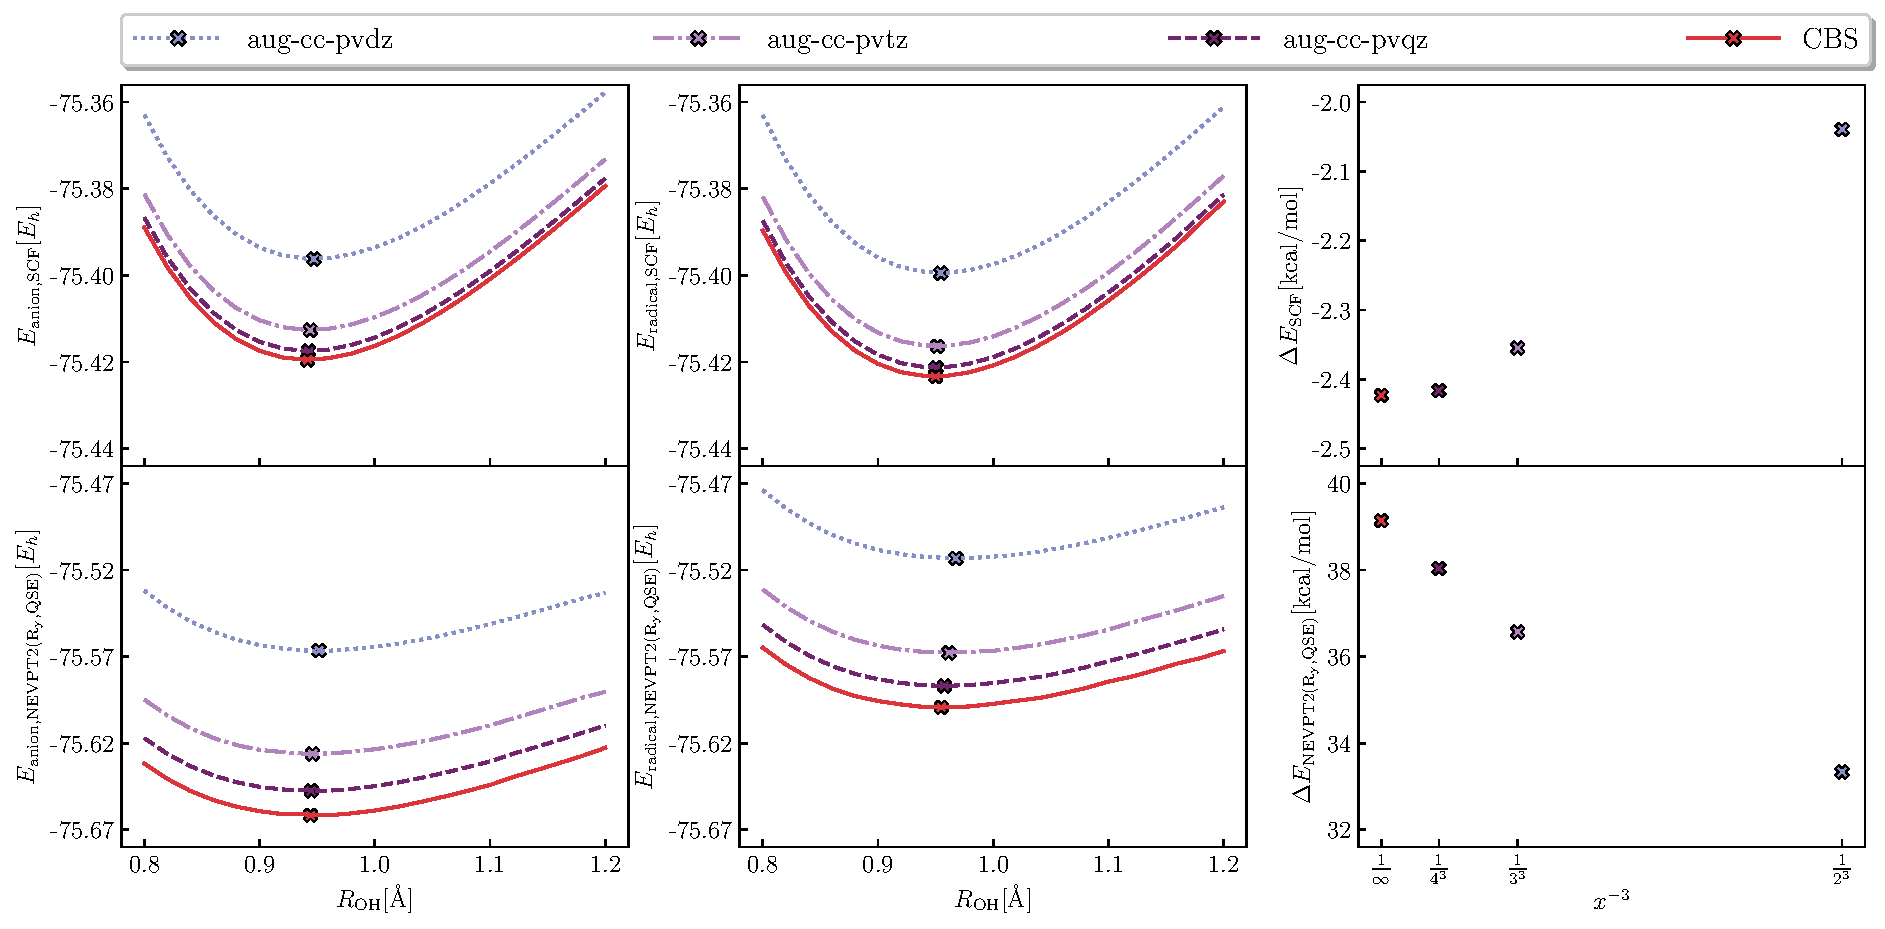
\includegraphics[width=0.75\textwidth]{../nevpt2/cbs_extrapolation/fig.pdf}
\caption{Potential energy curves of $\OHanion$ (anion, left) and  $\OHradical$ (radical, right) from Hartree-Fock (top) and NEVPT2(VQE,QSE)
using Dunning's aug-cc-pVxZ bases with x=D,T,Q (dotted, dot-dashed, and dashed lines respectively). 
Energies are extrapolated to the complete basis set (CBS, solid red lines) with standard procedures, and crosses denote equilibrium bondlengths and energies.}
\label{figure:dunning}
\end{figure*}

\begin{table*}[t!]
\begin{tabular}{lccc}
\hline\hline
method & $R_{\mathrm{anion}} [\mathrm{\AA}]$ & $R_{\mathrm{radical}} [\mathrm{\AA}]$ & $\Delta E$ [kcal/mol] \\ \hline
SCF,       & 0.94174(9) & 0.94994(34) & -2.423(35) \\
\hline
MP2 & 1.05604(19) & 1.05749(24) & 48.065(48) \\
CCSD & 1.05195(12) & 1.05723(15) & 37.908(31) \\
\hline
NEVPT2(R$_y$,QSE) & 0.93905(8) & 0.95349(32) & 34.311(29) \\
NEVPT2(q-UCCSD,QSE) & 0.93905(4) & 0.95336(23) & 34.284(20) \\
NEVPT2(FCI,QSE) & 0.93905(4) & 0.95336(22) & 34.273(19) \\
NEVPT2(FCI,FCI) & 0.96203(11) & 0.96252(13) & 39.188(15) \\
\hline\hline
\end{tabular}
\caption{Same as Table~\ref{tab:631g} with results extrapolated to the complete basis set limit (CBS).}
\label{tab:cbs}
\end{table*}

\subsection{Correlation-consistent augmented bases}

To address the basis set incompleteness error, in Fig.~\ref{figure:dunning} we perform simulations with correlation-consistent augmented bases aug-cc-pVxZ, $x=$D,T,Q or equivalently $2,3,4$.
Hartree-Fock and correlation energies are fit to the exponential Ansatz $E^{\mathrm{HF}}_x = a + b \, e^{-cx}$ with $x=2,3,4$ and and the power-law Ansatz $E^{\mathrm{c}}_x = a^\prime + b^\prime \, x^{-3}$ with
$x=3,4$ respectively. This standard procedure permits to extrapolate the energy to the complete basis set (CBS) limit as $E_{\mathrm{CBS}} = a+a^\prime$ \cite{feller1992application,helgaker1997basis}.

Equilibrium bondlengths and electron affinities extrapolated at CBS level of theory are reported in Table~\ref{tab:cbs}.
As seen, extrapolated equilibrium bondlengths from NEVPT2(FCI,FCI) are within 0.1 Angstrom from both CCSD and experimental values, 
and the QSE approximation introduces additional deviations, of order 0.01 $\mathrm{\AA}$.
Electron affinities from NEVPT2(FCI,FCI) and CCSD are within 1.2 kcal/mol from each other, and 3-4 kcal/mol away from the experimental value.
The QSE approximation causes an additional deviation of 5 kcal/mol from NEVPT2(FCI,FCI) results, which underestimates the electron affinity.

\section{Conclusion}
\label{sec:conclusions}

In this work, we integrated the VQE and QSE techniques in the workflow of the NEVPT2 method, and demonstrated such an inclusion
focusing on the relative stability of the hydroxide ion and hydroxyl radical. 
NEVPT2 allows for perturbative inclusion of dynamical correlation arising from non-valence orbitals, 
thereby improving the potential energy curves produced by quantum computing simulations limited to valence spaces.

The main limitation of such simulations is that electronic correlation is captured within a valence space only. 
Therefore, perturbative or full inclusion of virtual orbitals is necessary to cover the dynamical correlations with methods like coupled cluster and multireference configuration interaction model, and very important to obtain quantitative agreement with experimental values, especially for sensitive quantities such as polarizabilities or thermochemical properties.

We expect that the perturbative inclusion of dynamical correlation from external orbitals, 
as a technique to partially overcome the limitations of minimal basis sets and active spaces, 
will prove useful in the simulation of chemical species by quantum algorithms on contemporary quantum devices.

\section*{Acknowledgments}

AT, DEG and MM acknowledge the Universit\`a degli Studi di Milano INDACO Platform and the IBM Research Cognitive Computing Cluster service respectively, 
for providing resources that have contributed to the results reported within this study.

\section{Computational details}

In this Appendix, we provide additional details about the computational methods used in the present work.

\subsection{Orbital construction}
\label{app:orbitals}

In this Subsection, we describe the construction of core, active, and external orbitals. First, we fix an underlying basis of atomic orbitals 
(AOs). We then perform a Hartree-Fock calculation of restricted type, yielding a set of molecular orbitals (MOs) and a Fock operator 
$\hat{F} = \sum_a f_a \crt{a\sigma} \dst{a\sigma}$.

Then, from the MOs, we construct a set of intrinsic atomic orbitals (IAOs), specified by coefficients $C^{\mathrm{IAO}}_{p\mu}$, using standard procedures. 
It is important to remarkthat IAOs span occupied MOs and the valence region of the underlying basis.
We perform a second Hartree-Fock calculation of restricted type in the IAO basis, leading to a set of MO coefficients $C_{\mu k}$
and to a corresponding set of. molecular orbitals $C^{\mathrm{MO}}_{pk} = \sum_{\mu} C^{\mathrm{IAO}}_{p\mu} C_{\mu k}$.

These MOs are orthonormal, have a clearly occupied or virtual (i.e. unoccupied) character, and span the same subspace as the IAOs, 
corresponding to the valence region of the underlying basis.
The low-energy and doubly occupied MOs serve as the core orbitals,
\begin{equation}
\label{eq:orb1}
C^{\mathrm{core}}_{pi} = C^{\mathrm{MO}}_{pi} \;,\; i=1 \dots N_f \;,
\end{equation}
and their number $N_f$ is determined by the atomic species in the molecule. The remaining MOs serve as active orbitals,
\begin{equation}
\label{eq:orb2}
C^{\mathrm{act}}_{pu} = C^{\mathrm{MO}}_{p N_f+u} \;,\; u= 1 \dots N_{\mathrm{IAO}}-N_f \;.
\end{equation}
To determine the external orbitals, we form the projector 
\begin{equation}
\Pi_{pr} = \sum_{kq} C^{\mathrm{MO}}_{pk} C^{\mathrm{MO}}_{qk} S_{qr}
\end{equation}
on the subspace spanned by core and active orbitals, where $S_{qr}$ is the overlap matrix in the AO basis,
and the projector $\Lambda = \mathbbm{1}-\Pi$ onto its orthogonal complement.
We then project the Fock operator onto the orthogonal complement of the core+active space,
$\tilde{F} = \Lambda F \Lambda$, diagonalize such operator, and define external orbitals
as the eigenvector of $\tilde{F}$ in the null space of $\Pi$,
\begin{equation}
\label{eq:orb3}
\begin{split}
\sum_r \tilde{F}_{pr} C^{\mathrm{ext}}_{ra} &= \varepsilon_a C^{\mathrm{ext}}_{pa} \; , \\
\sum_r \Pi_{pr} C^{\mathrm{ext}}_{ra} &= 0 \; . \\
\end{split}
\end{equation}
Equations \eqref{eq:orb1}, \eqref{eq:orb2}, and \eqref{eq:orb3} correspond to the core, active, and external orbitals respectively.

\subsection{Core freezing}
\label{app:core}

In this Subsection we report, for completeness, the frozen-core procedure used to remove core orbitals from the simulation.
With the indices $i,j$ and $p,r,q,s$ we respectively denote core and non-core (active or external) orbitals.
\begin{equation}
\begin{split}
\hat{H} &= E_0 + \sum_i 2 h_{ii} + \sum_{\substack{ pr \\ \sigma}} h_{pr} \crt{p\sigma} \dst{r\sigma} \\
&+ \sum_{ij} 2(ii|jj) - (ij|ji) \\
&+ \sum_{\substack{ pr \\ \sigma}} \Big[ (pr|ii) - (ir|pi) \Big] \crt{p\sigma} \dst{r\sigma} \\
&+ \sum_{\substack{ prqs \\ \sigma\tau}} \frac{(pr|qs)}{2} \crt{p\sigma} \crt{q\tau} \dst{s\tau}  \dst{r\sigma} \;.
\end{split}
\end{equation}
The Hamiltonian can then be written as in Eq.~\eqref{eq:core_frozen} with
\begin{equation}
\begin{split}
E_0^\prime &= E_0 + \sum_i 2 h_{ii} + \sum_{ij} 2(ii|jj) - (ij|ji) \\
t_{pr} &= h_{pr} + \sum_i (pr|ii) - (ir|pi) \\
v_{prqs} &= (pr|qs) \\
\end{split}
\end{equation}

\begin{figure*}[t!]
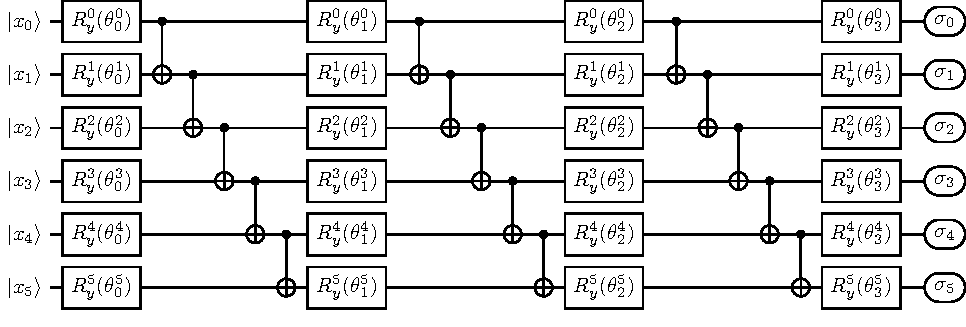
\includegraphics[width=0.6\textwidth]{quantum_circuit/figure-figure0.pdf}
\caption{Quantum circuit describing the $R_y$ Ansatz with depth $n_r=3$ acting on $n_q=4$ qubits.}
\label{fig:ry}
\end{figure*}

\subsection{Computation of transition matrix elements}
\label{app:transition}

In this Subsection, we detail the computation of the transition matrix elements in Eq.~\eqref{eq:nevpt5}. 
In general, to achieve this goal one has to measure additional operators on a quantum computer.
When Eq.~\eqref{eq:nevpt6} is adopted, on the other hand, the outcomes of these additional measurements are trivially related to the QSE overlap matrices.
First,
\begin{equation}
\label{eq:omega_1}
\begin{split}
\Omega^\sigma_{\mu,a} 
&= \langle \Phi^{(\sigma)}_\mu | \hat{O}^{(1)}_{a,\sigma} | \Phi_0 \rangle = \sum_u \chi_{u\mu}^\sigma \langle \Phi_0 | \crt{u\sigma} \hat{O}^{(1)}_{a,\sigma} | \Phi_0 \rangle \\
&= \sum_u \chi_{u\mu}^\sigma \left[ \sum_{y} t_{ay} \, \rho^\sigma_{uy}  + \sum_{ \substack{ywz \\ \tau} } v_{aywz} \, \rho^{\sigma\tau}_{uywz} \right] \\
\end{split}
\end{equation}
where we introduced the spin-resolved one- and two-body density matrices. Similarly,
\begin{equation}
\label{eq:omega_2}
\begin{split}
\Omega^{\sigma\sigma}_{\mu,ab} 
&= \langle \Phi^{(\sigma\sigma)}_\mu | \hat{O}^{(2)}_{ab,\sigma} | \Phi_0 \rangle \\
&= \sum_{u<v} \chi_{uv,\mu}^\sigma \langle \Phi_0 | \crt{v\sigma} \crt{u\sigma} \hat{O}^{(2)}_{ab,\sigma} | \Phi_0 \rangle \\
&= \sum_{u<v} \chi_{uv,\mu}^\sigma \, \left[ \sum_{xy} v_{aybx} \, \rho^{\sigma\sigma}_{vyux} \right] \quad. \\
\end{split}
\end{equation}
Finally,
\begin{equation}
\label{eq:omega_3}
\begin{split}
\Omega^{\uparrow\downarrow}_{\mu,ab} 
&= \langle \Phi^{(\uparrow\downarrow)}_\mu | \hat{O}^{(3)}_{ab} | \Phi_0 \rangle \\
&= \sum_{uv} \chi_{uv,\mu}^\sigma \langle \Phi_0 | \crt{v\downarrow} \crt{u\uparrow} \hat{O}^{(3)}_{ab} | \Phi_0 \rangle \\
&= \sum_{uv} \chi_{uv,\mu}^\sigma \, \left[ \sum_{xy} v_{aybx} \, \rho^{\uparrow\downarrow}_{vyux} \right] \quad .\\
\end{split}
\end{equation}
We can now observe that one- and two-body density matrices are trivially related to the QSE overlap matrices. 
Indeed,
\begin{equation}
\begin{split}
\rho^\sigma_{uy} 
&= \langle \Phi_0 | \crt{u\sigma} \dst{y\sigma} | \Phi_0 \rangle = S^\sigma_{uy} \quad, \\
\end{split}
\end{equation}
and similarly

\pagebreak % attenzione

\begin{equation}
\begin{split}
\rho^{\sigma\sigma}_{uywz} 
&= \langle \Phi_0 | \crt{u\sigma} \crt{w\sigma} \dst{z\sigma} \dst{y\sigma} | \Phi_0 \rangle \\
&= (-1)^{\delta_{w w^\prime}+\delta_{z z^\prime}} \, \langle \Phi_0 | \crt{u^\prime\sigma} \crt{w^\prime\sigma} \dst{z^\prime\sigma} \dst{y^\prime\sigma} | \Phi_0 \rangle \\
&= (-1)^{\delta_{w w^\prime}+\delta_{z z^\prime}} S^{\sigma\sigma}_{(w^\prime u^\prime),(z^\prime y^\prime)} \quad, \\
\rho^{\uparrow\downarrow}_{uywz}  
&= \langle \Phi_0 | \crt{u\uparrow} \crt{w\downarrow} \dst{z\downarrow} \dst{y\uparrow} | \Phi_0 \rangle = S^{\uparrow\downarrow}_{(wu),(zy)} \quad, \\
\end{split}
\end{equation}
where

\begin{equation}
\begin{split}
w^\prime &= \mbox{min}(u,w) \quad, \\
u^\prime &= \mbox{max}(u,w) \quad, \\
z^\prime &= \mbox{min}(z,y) \quad, \\
y^\prime &= \mbox{max}(z,y) \quad. 
\end{split}
\end{equation}
The cost of computing Eq.~\eqref{eq:omega_1} and (\ref{eq:omega_2}-\ref{eq:omega_3}) is respectively of $\mathcal{O}(N_{ext} N_{act}^3 + N_{ext} N_{act} N_{qse})$,
and  $\mathcal{O}(N^2_{ext} N_{act}^4 + N^2_{ext} N^2_{act} N_{qse})$ operations.

\subsection{$R_y$ variational form}
\label{app:ry}

The quantum circuit defining the variational form used in the present work is shown in Fig.~\ref{fig:ry}.

The initial state $|x_0 x_1 x_2 x_3 \rangle$ is the computational basis state (i.e. a tensor product of eigenstates of the $Z$ Pauli operator)
representing the Hartree-Fock state in presence of tapering. For the anion and radical, this is respectively $(x_0,x_1,x_2,x_3)=(0,1,1,0)$
and $(x_0,x_1,x_2,x_3)=(0,1,0,0)$.
Observables such as the active-space Hamiltonian $\hat{H}_{act}$ and the QSE overlap and Hamiltonian operators $\hat{E}_\alpha^\dagger \hat{E}_\beta$,
$\hat{E}_\alpha^\dagger \hat{H}_{act} \hat{E}_\beta$ are represented as linear combinations of Pauli operators $P = \otimes_{i=0}^{n_q-1} \sigma_i$.

At the end of the circuit, Pauli operators $P$ are measured, and the results of these measurements are used to compute expectation values of relevant 
operators using standard techniques \cite{aleksandrowicz2019qiskit}.

\bibliographystyle{apsrev4-2}
\bibliography{main}

\end{document}
